\chapter*{Introduction générale}

\begin{itemize}
	\item Ici on parlera des motivations qui ont aboutis à ce projet, des objectifs de ce dernier ainsi que ses perspectives
\end{itemize}


\chapter{Assistants virtuels intelligents}

\section{Introduction}
\paragraph{}
Depuis la commercialisation du premier ordinateur grand public(\textbf{Xerox PARC Alto}) en 1973, le monde découvris pour la première fois ce qui allait devenir l'apparence basique de chaque ordinateur moderne, en effet ils furent les premiers à proposer une interface graphique dotée de fenêtres, d'icônes et d'uns souris pour se déplacer et d'un clavier pour écrire du texte. Bien que basique, cette idée lança alors plusieurs autres grandes marque sur le même chemin (IBM,Apple,Compaq ...), Par la suite beaucoup ont essayé d'améliorer la façon dont l'homme utilisait sa machine : souris plus précise, écran doté d'une plus grande résolution, clavier plus enrichis, voir même l'introduction des écrans tactiles dans certains systèmes embarqués.
\par Cependant, certains voyaient encore cette façon d'utiliser la machine comme \textbf{trop primitive}, et peu intuitive, en effet laisser un enfant devant un ordinateur et il prendrait un bon moment pour apprendre à ne serait ce qu'éditer un simple fichier. pour citer Donald A. Norman 
\begin{quote}
	\say{We must design for the way people behave, not for how we would wish them to behave.}\cite{don-norman}
\end{quote}
Traduit par :
\begin{quote}
	\say{Nous devons concevoir selon le comportement des utilisateurs, et non pas selon la façon dont nous voudrions qu'ils se comportent.}
\end{quote} 
L'humanité à fait beaucoup de chemin depuis les années 70, utiliser un ordinateur de nos jours avec les moyens \textbf{classiques} (souris, clavier, écran ...) est devenu une tâche triviale, voir même une seconde nature, ça reste cependant dû au fait que de plus en plus de jeunes enfants sont exposés depuis leur plus jeune âge au monde technologique qui les entoure, le processus d'apprentissage reste cependant présent, l'effort d'utiliser les outils communs reste lui aussi présent.
\par Qu'on le veuille ou pas, la plus naturelle et plus ancienne façon de communiquer pour l'homme à toujours été la parole, l'invention de langues toutes aussi riches et complexes les unes que les autres à permis à l'humanité de briser plusieurs barrières sociales. l'avancement le plus naturel pour cette façon de communiquer serait donc de l'étendre non plus seulement qu'aux humains, mais aussi aux machines que l'homme ç su construire et améliorer au fil des années.
\par 
Motivé par cette manière que l'on a de communiquer entre nous, et épaulé par les récentes technologies tel que l'apprentissage automatique\ref{Section2} et le traitement automatique du langage naturel\ref{Section2} et de l'intelligence artificielle en tant que tout un domaine, les plus brillants des chercheurs ont entamé leurs recherches dans un tout nouveau domaine.
\par 
Les Assistants Virtuels Intelligents sont donc le produit de plusieurs années de recherche, visant tout d'abord à faciliter certaines tâches pour l'utilisateur, les premiers AVI était conçu comme des agents de conversation ou \textbf{Chatbots}, limités dans leurs actions et dépendant toujours d'un moyen de communication textuel, ce ne fut pas la forme désirée de l'AVI par excellence, avec l'avancement des recherches sur la reconnaissance automatique de la parole et l'émergence de l'apprentissage automatique ( les tout premiers assistant virtuels utilisant la RAP étant spécialisés dans certains domaines comme des système d'aides à la décision médicaux ), il a ensuite été plus aisé de briser la barrière et de réaliser ce qui était encore une esquisse d'un AVI personnalisé avec l'émergence de l'apprentissage profond(\ref{Section2}) et la popularisation des Smartphones\footnote{Text about smartphones here }, de nouveaux AVIs comme \textbf{Apple Siri}\ref{siri} en 2011 et \textbf{Google assistant} et \textbf{Amazon Alexa} ont fait leur apparitions, offrant de plus en plus de services personnalisés et spécifiques à chaque utilisateurs.
Dans la suite de ce chapitre nous essayerons de mieux détailler ce qu'est un AVI, ce qui est demandé d'un tel système, des différents types d'AVIs et des domaines d'application de ces derniers, pour enfin  conclure sur les limitations actuelles et les motivations de ce projet. 

\newpage
\section{Un robot à tout faire}\label{spa-def}
Informellement, un AVI est type d'\textbf{agent\footnote{un agent est ...}} logiciel qui peut effectuer certaines tâches et proposer des services dédiés aux utilisateurs qui vont d'une simple tâche (Ouvrir une fenêtre, lancer une application ...) à la réalisation de requêtes un peu plus complexes ().
Pour répondre efficacement à toutes sortes de requêtes, un AVI se doit donc de garder trace du contexte courant de sa conversation avec l'utilisateur, il doit donc disposer d'un système capable d'enregistrer les informations pertinentes et de savoir les réutiliser, mais aussi de pouvoir déduire les quelles de ces informations sont manquantes, on parle ici de Context-Awarness ou Sensibilité au contexte, comme vu dans \cite{SPA-overview}.
\par toujours d'après \cite{SPA-overview} et \cite{Dey-Abwod}
\textit{Day} et \textit{Abwod} définissent un contexte comme suit : 
\begin{quote}\label{context-def}
	\say{A context is any information
		that can be used to characterize the situation of an entity. An entity is a person, place,
		or object that is considered relevant to the interaction between a user and an
		application, including the user and applications themselves}
\end{quote}
Qui peut être traduit par :
\begin{quote}\label{context-def-fr}
	\say{Un contexte est une information qui peut être utiliser pour caractériser l'état d'une entité. Un entité peut être une personne une place ou un objet considéré comme pertinent vis à vis de l'interraction entre l'utilisateur et l'application, ainsi que ces deux derniers en eux mêmes}
\end{quote}
Il en découle que pour parvenir à développer un système qui puisse répondre aux besoins individuels et spécifiques de chaque personne, parvenir à modéliser et prendre en compte le contexte semble être une solution prometteuse.

\section{Architecture générale d'un AVI}
\paragraph{}
Il n'existe pas vraiment d'architecture type pour un AVIs, chaque équipes de chercheurs à tenté sa propre implémentation, il existe en revanche une représentation haut-niveau des composants d'un tel système, nous proposons à titre d'exemple la pseudo-architecture interne de l'assistant de Google : 
\begin{figure}[H]
	\centering
	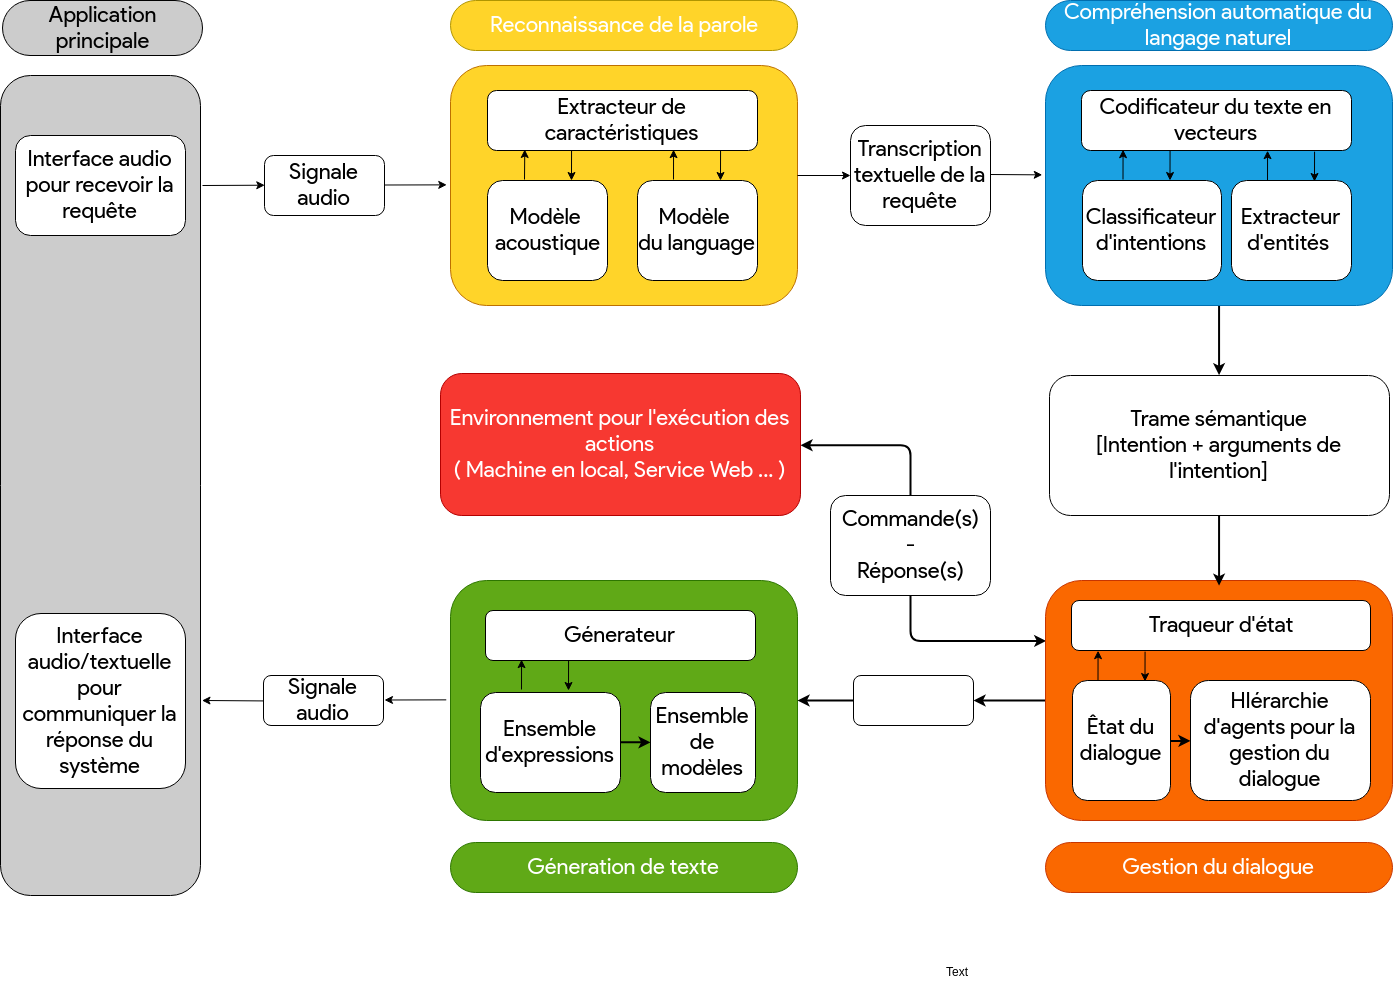
\includegraphics[width=\linewidth]{images/SPA_architecture.png}
	\caption{Architecture haut niveau de Google Assistant \cite{GAlayout}}
\end{figure}
On peut ainsi dégager le schéma simplifié abstrait suivant : 
\begin{figure}[H]
	\centering
	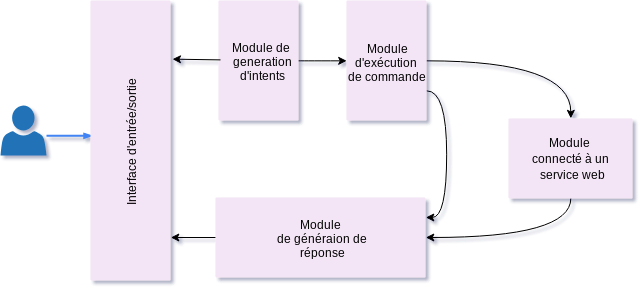
\includegraphics[width=\linewidth]{images/SPA_diagram.png}
\end{figure}

\section{Caractéristiques principales d'un AVI}
\subsection{Sensible au contexte}
\paragraph{}
Comme précédemment vu dans la définition du contexte (voir \ref{context-def}), ce dernier peut être interprété comme tout aspect d'une entité(Position d'un objet, couleur d'un objet, température d'une chambre ..etc ), Un assistant dit \textbf{intelligent} doit donc être capable de capturer le concept du contexte, d'utiliser et de traiter toute informations catégorisée comme contextuelle.
Pour être plus précis, l'AVI doit être sensible à \textit{l'évolution} du contexte courant, par le biais de capteur optiques de microphones .. etc, tout ce qui pourrait amener l'utilisateur à faire évoluer la demande qu'il à émis, l'assistant devra donc proposer un système de mise à jours du contexte pour éliminer les informations inutiles et garder celles qui pourraient aider à répondre à la requête de l'utilisateur.
\subsection{Évolutif}
\paragraph{}
Il a été vu dans \ref{spa-def} qu'un AVI peut être vu comme un type d'agent. Pour rappel d'après \textit{Russel} et \textit{Norvig} un agent (qui est une entité autonome pouvant interagir avec son environnement afin d'accomplir certaines tâches) peut être de plusieurs types : 
\begin{itemize}
	\item Agent simple réflexe : agent exécutant ses actions à base de règle conditionnelles simple (c.à.d \textbf{Si} \textit{Condition } \textbf{alors} \textbf{exécuter actions}), ils sont ainsi très simplistes et limité dans la porté de leur actions.
	
	\item Agent basé modèle : semblables aux agents simple réflexe, il sont toute fois doté d'un modèle interne complexe sensé représenté le monde extérieur auquel l'agent à accès, cependant ils appliquent les actions de la même manière que le précédent type d'agents.
	
	\item Agent à but : un amélioration des agents simple qui sont dotés d'un ensembles d'états buts à atteindre d'une façon ou d'une autre
	
	\item Agent à utilité : des agents à buts qui tentent d'aboutir à leurs buts d'une manières optimisée (intelligente) utilisant une fonction de de mesure adéquate pour le choix des différents états à atteindre.
	
	\item Agent apprenant : agent à utilité enrichi par un module d'apprentissage qui sert de juge pour répondre aux \textbf{"critiques"} des actions qu'il entreprenant, le terme \textbf{agent évolutif} est aussi employé.
\end{itemize}
\par Pour ce qu'il en est des AVIs, les plus récents systèmes (ex : \textbf{Amazon Alexa} qui améliore so  module de reconnaissance de la parole après chaque réponses non déclinée par l'utilisateur), peuvent être considérés comme des agent apprenants, répondant de ce fait à la contrainte évolutive imposée, cependant le domaine de l'auto-évolution des systèmes intelligent est encore un domaine nouveau qui se voit épaulé par les récentes avancées dans le domaine de l'apprentissage automatique \cite{SPA-overview}


\subsection{Multimodal }
\paragraph{}
Afin d'assurer une aisance d'utilisation, les AVI's sont fréquemment amenés à récupérer les requêtes(ou données) en entrée de la manière la plus naturelle possible(par exemple par le biais de la paroles). Cependant, pour garantir une expérience d'utilisation adéquate, l'assistant sera souvent confronté à récupérer ses requêtes de différentes manières, que ce soit à travers une interface graphique(écran tactile) ou à travers d'un texte brut tapé au clavier voir même à travers des expressions faciales ou des états cognitives/émotionnels (\cite{Dingler2016}), pour ensuite produire une réponse qui, elle aussi pourrait éventuellement être de la forme textuelle ou sonore ou les deux ..., cette capacité à recevoir en entrée et/ou produire une sortie de plusieurs façon différentes est la multi-modalité d'après \cite{Luger2016}, et cette caractéristique qui permet de masquer à l'utilisateur toute la complexité d'acquisition de ses requêtes.

\subsection{Anthropomorphe}\label{antropo}
\paragraph{}
Plusieurs auteurs tendent à attribuer une grande importance à l'anthropomorphisme des AVIs (\cite{virtualbutler}), qui est 
\begin{quote}
	\say{Un mécanisme qui pousse les êtres humains à induire qu'une entité non-humanoïde possède des caractéristiques et comportements propres à l'homme}\cite{alexabff}
\end{quote}

\par Ce comportement humanoïde pousserait donc l'utilisateur à se sentir plus à l'aise avec l'assistant, le conduisant ainsi à adopter une façon de communiquer plus humaine et moins structuré qu'avec les les autres machines, c'est ainsi une caractéristiques majeure d'un AVIs se disant \textbf{personnalisé}.
\subsection{Multi plateforme et Flexible }
\paragraph{}
Malgré leur récentes prouesses, certains AVIs sont encore restreints à un écosystème fortement dépendant du fabricant,  Cowan et al. mentionnent dans \cite{Cowan2017} que Apple Siri est limité à l'environnement constitué des produits de la firme à la pomme, n'ouvrant par défaut que les applications de cette dernière quand une requête lui est transmise.
\par C'est un comportement que les assistants devrait éviter, car une indépendance des plateformes utilisées est, certes, très complexe à instaurer, mais offre plus de possibilités aux utilisateurs et aux développeurs, pouvant ainsi exploiter la puissance de certaines plateformes(Smartphones, TV connectées ...).
Avec l'émergence de l'IoT(Internet of Things) et des maisons intelligentes  par exemple, c'est un tout nouveau terrain de jeu qui est présenté pour les AVI's, offrant plus d'opportunités pour les utilisateurs.
\section{Domaines d'applications des AVIs}
\paragraph{}
Après avoir vu les différents aspects que les AVIs doivent traiter, nous nous intéresserons maintenant aux types de services et applications que ces derniers pourraient fournir pour démontrer qu'ils peuvent bel et bien faciliter certaines tâches à l'homme.

\subsection{Vie quotidienne}
\paragraph{}
À la base, les AVIs étaient destinés à un usage très personnel comme la gestion des achats dans les supermarchés, ou des guides touristiques de plusieurs destinations de voyage, cette spécificité à commencé a s'estompé petit à petit avec l'émergence de nouveaux systèmes dédiés à des applications plus générales, comme les maisons intelligentes ou les assistant de planifications de tâches, ce qui à permit de mettre encore plus l'accent sur cet aspect de convivialité que les tout premiers AVIs en tenter de perfectionner, ainsi tout ces assistants spécialisés dans des domaines restreints(Tourisme, shopping, détente ...)   sont regroupés dans un seul système plus polyvalent capable de répondre à des besoins quotidiens divers et variés, allant même à fournir une assistance aux personnes âgées pour leur faciliter les tâches rudimentaires devenues trop fatigantes  
\subsection{Assistance professionnel}
\paragraph{}

\subsection{E-enseignement}
\paragraph{}


\section{Types d'assitants virtuel}
\paragraph{}

\subsection{ChatBot(Agent de conversation)}
\label{chatbot}
\subsection{Virtual Administrative Assistant}
\subsection{Social Media Marketing Virtual Assistant}
\subsection{Virtual Assistant Writers}
\subsection{Virtual Research Assistant}
\subsection{eCommerce Virtual Assistant}
\subsection{Data Entry Virtual Assistant}

%\begin{itemize}
%	\item ChatBot(Agent de conversation)
%	\item Virtual Administrative Assistant
%	\item Social Media Marketing Virtual Assistant
%	\item Virtual Assistant Writers
%	\item Virtual Research Assistant
%	\item eCommerce Virtual Assistant
%	\item Data Entry Virtual Assistant
%\end{itemize}

\hl{
	`interesring links : `
	[first](https://www.acelerartech.com/va-guide/types-of-virtual-assistant-services/)
	[second](http://outsourceworkers.com.au/different-kinds-of-virtual-assistants/)}


\newpage
\section{Exemples d'AVI}
\paragraph{}
Pour illustrer la puissance des AVIs les plus récents, nous avons décidé de mettre en évidence les quatre produits qui dominent le marché courant :

\subsection*{Google assistant}
\paragraph{}
\begin{figure}[H]
	\centering
	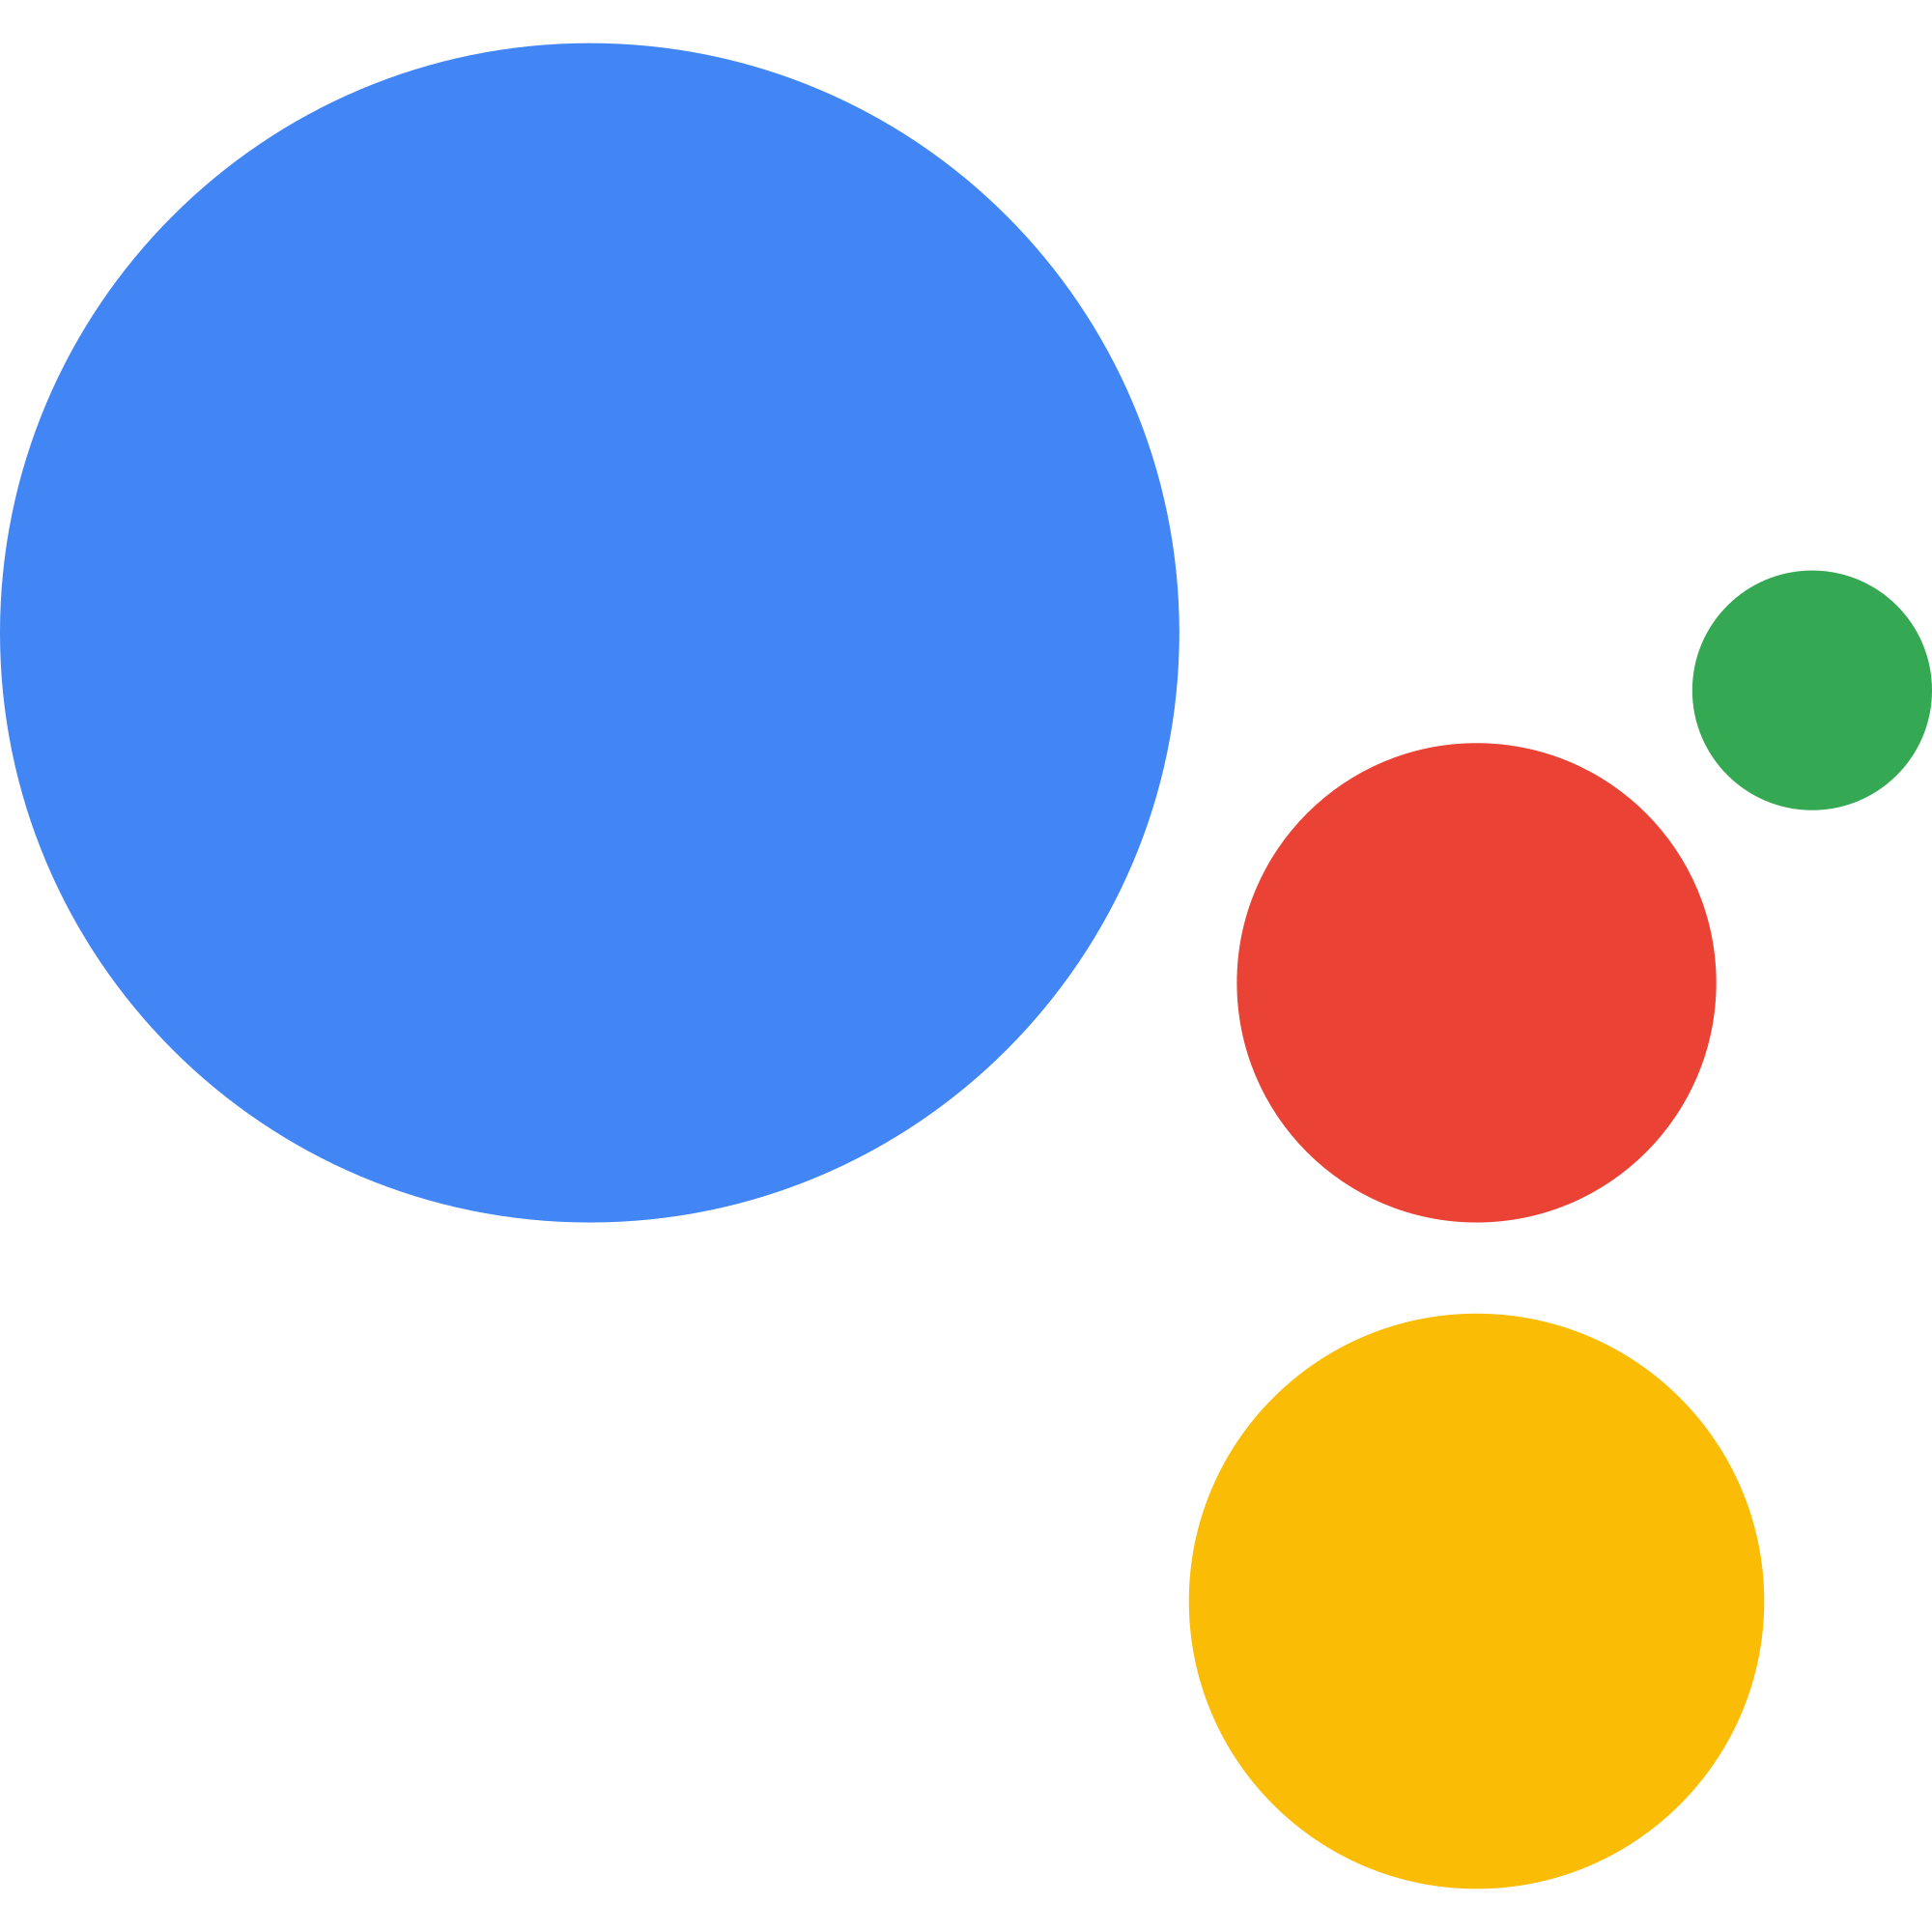
\includegraphics[width=.2\linewidth]{images/google_assitant/logo.png}
	\caption{Logo de Google assistant} 
\end{figure}
Lancé en 2016 comme un chatbot(\ref{chatbot})intégré dans l'application Google Allo, G.A s'est vu ensuite être directement intégré sur les système d'exploitation Android(que ce soit sur smartphones ou tablettes, et plus récemment sur Google Home\footnote{Appareil servant à contrôler les composant d'une smart-house ainsi que l'utilisation des différents services de google} ), G.A est un assistant à tout faire concocter par les ingénieurs de Google dans le but de faciliter la recherche sur internet, la planification des tâches, l'ajustement des réglages de l'appareil ..., sont point fort est sa capacité à engager une conversation bi-directionnel avec l'utilisateur, assurant ainsi une interaction personnalisé variant d'un utilisateur à un autre, cela lui permet par exemple de proposer certains résultats de recherche selon les les précédentes interactions avec l'utilisateur, ou de luis proposer une activité si ce dernier lui reproche de s'ennuyer.
\begin{figure}[H] 
	\label{ fig7} 
	\begin{minipage}[b]{0.5\linewidth}
		\centering
		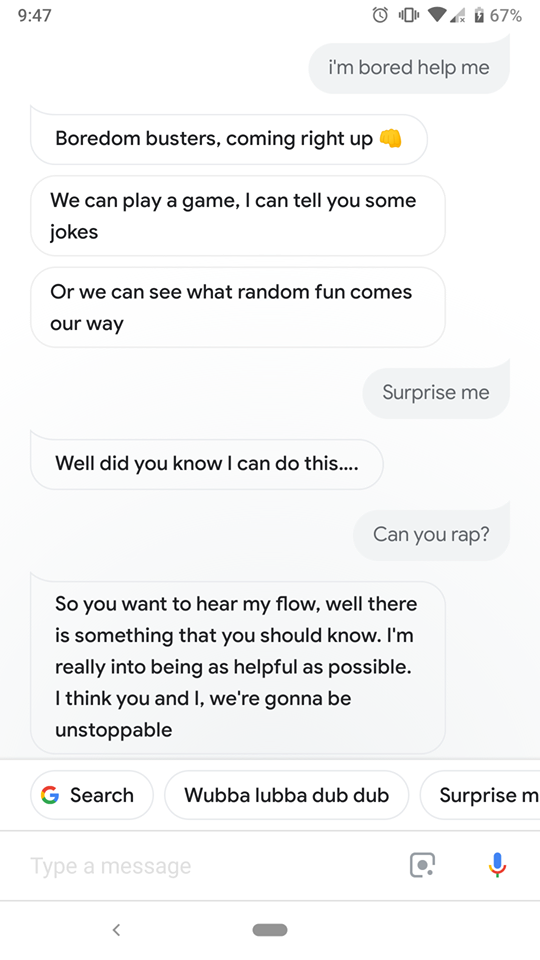
\includegraphics[width=.5\linewidth]{images/google_assitant/bored.png} 
		\caption{Conversation aléatoire 1} 
		
	\end{minipage}%%
	\hfill
	\begin{minipage}[b]{0.5\linewidth}
		\centering
		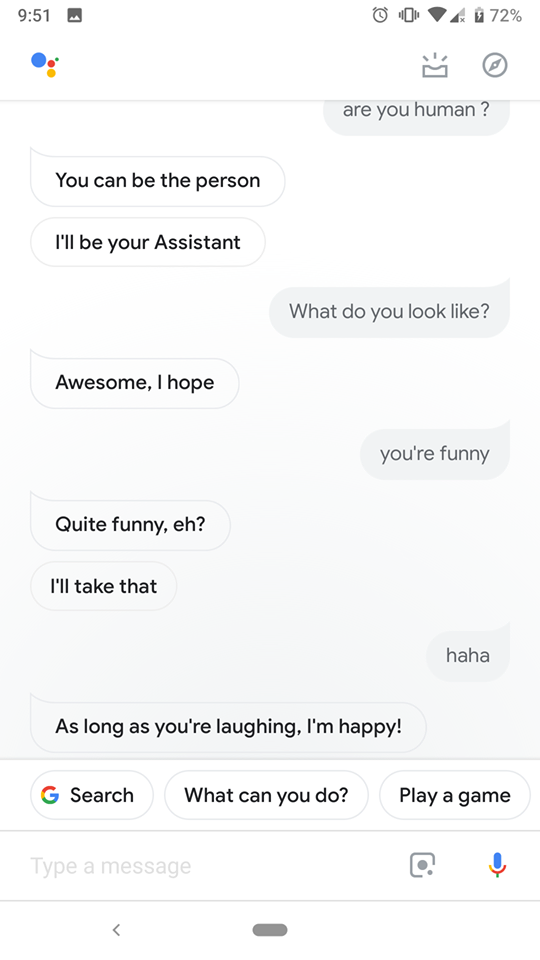
\includegraphics[width=.5\linewidth]{images/google_assitant/humanlike.png} 
		\caption{Conversation aléatoire 2} 
		
	\end{minipage} 
	\begin{minipage}[b]{0.5\linewidth}
		\centering
		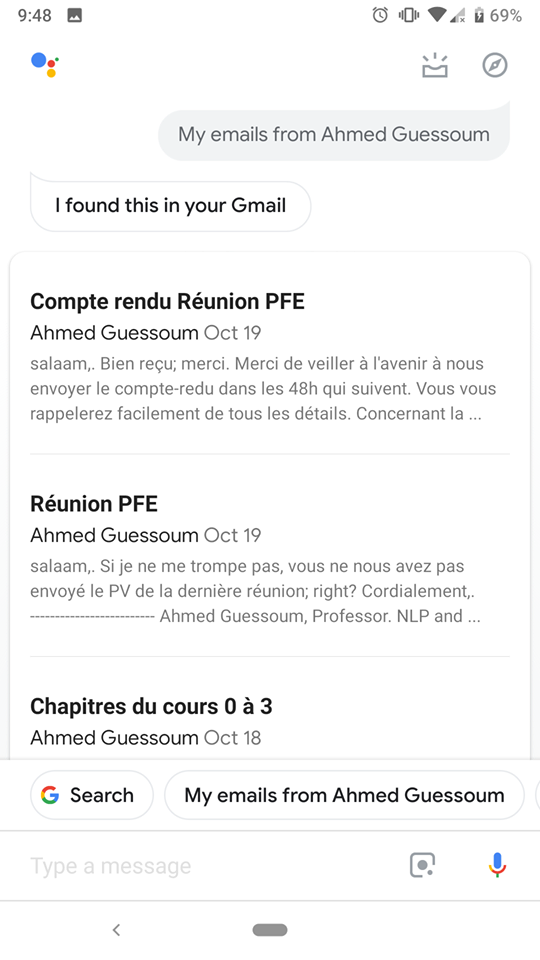
\includegraphics[width=.5\linewidth]{images/google_assitant/mails.png} 
		\caption{Requête simple 1} 
		
	\end{minipage}
	\hfill
	\begin{minipage}[b]{0.5\linewidth}
		\centering
		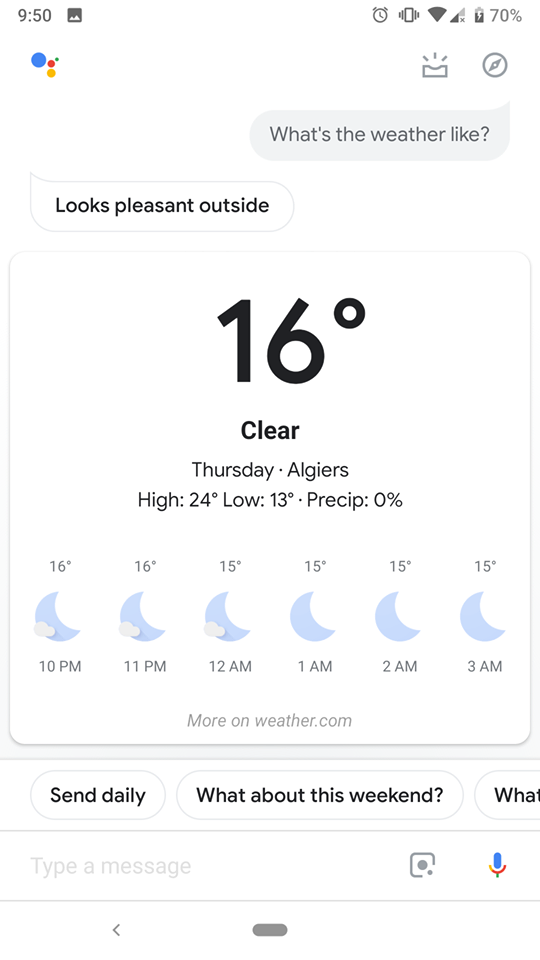
\includegraphics[width=.5\linewidth]{images/google_assitant/weather.png} 
		\caption{Requête simple 2} 
		
	\end{minipage} 
\end{figure}


\subsubsection*{Google duplex}
\begin{figure}[H]
	\centering
	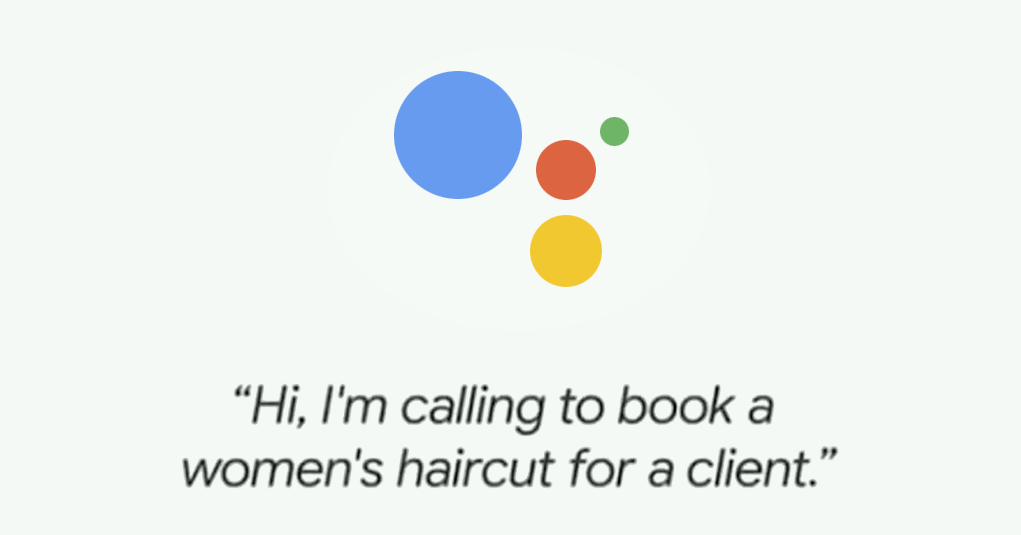
\includegraphics[width=.5\linewidth]{images/google_assitant/duplex.png} 
	\caption{Google duplex en réservant une place dans un salon de coiffure} 
\end{figure}
\par une des nouveautés impressionnante de G.A est la fonctionnalité Google Duplex, toujours en phase de développement, ce module est capable de passer des appels a de vrais personnes et d'avoir une conversation avec elles afin de réaliser une tâche demandé par l'utilisateur comme par exemple réserver une chambre d'hôtel, une table au restaurant ... 



\subsection*{Apple Siri}
\begin{figure}[H]
	\centering
	
\includegraphics[width=.25\linewidth]{images/apple_siri/logo.png}
	\caption{Logo d'Apple Siri} 
\end{figure}
\paragraph{}
Siri est l'assistant virtuel développé par Apple, contrairement au AVIs durant sa sortie, Siri proposait une nouvelle façon de communiquer avec l'utilisateur, proposant une interface de requêtes vocale, et une façon de communiquer très humanoïde (satisfaisant ainsi le critère d'anthropomorphisme voir \ref{po}).
Siri est capable de répondre à des questions précises, de proposer des recommandations, ou bien déléguer la requête à des services web. Il à l'avantage(et l'inconvénient) d'être disponible sur la multitude des appareils qui composent l'écosystème d'Apple (MacBook,iPhone,iWatch ...).

\begin{figure}[H] 
	\begin{minipage}[b]{0.45\linewidth}
		\centering
		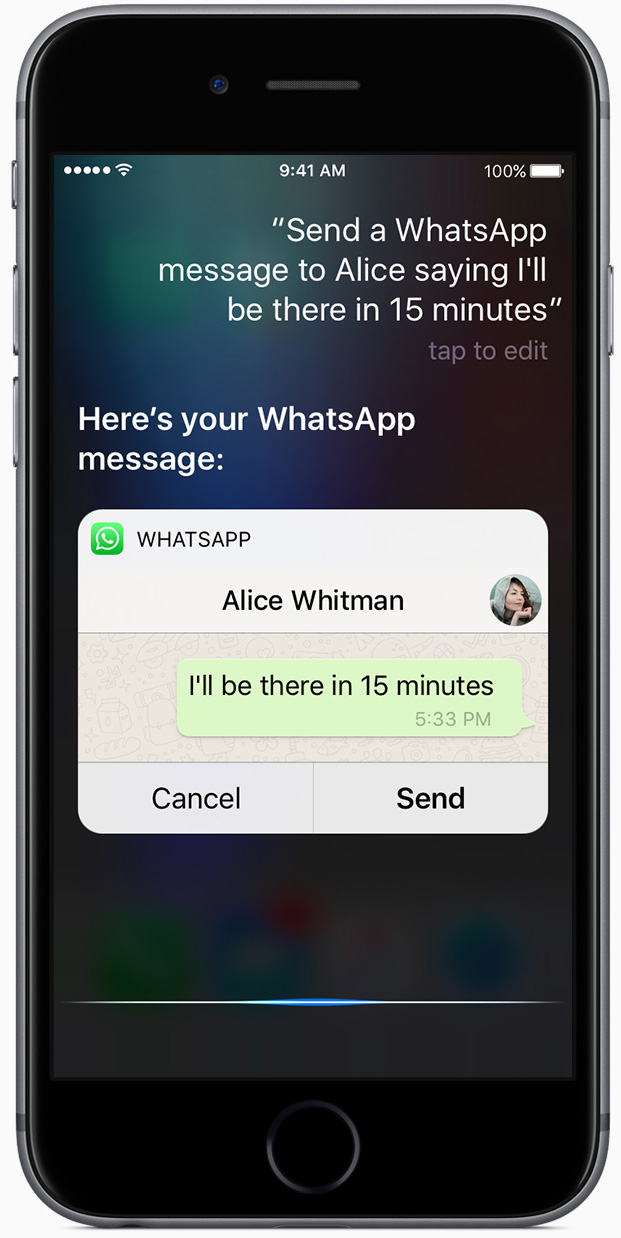
\includegraphics[width=.5\linewidth]{images/apple_siri/whatsapp.jpg} 
		\caption{Intégration aux applications 1 \cite{siriDemo}} 
		%	
	\end{minipage}%%
	\hfill\hfill
	\begin{minipage}[b]{0.45\linewidth}
		\centering
		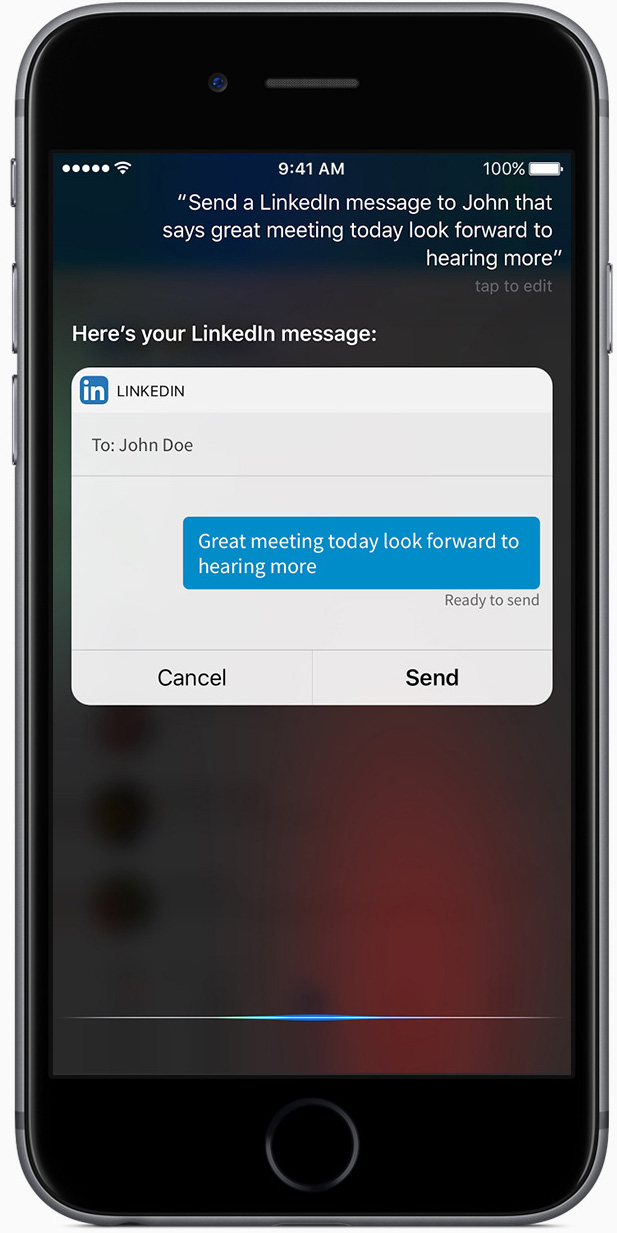
\includegraphics[width=.5\linewidth]{images/apple_siri/linkedin.jpg} 
		\caption{Intégration aux applications 2 \cite{siriDemo}} 
		
	\end{minipage} 
\end{figure}

\begin{figure}[H]
	\centering
	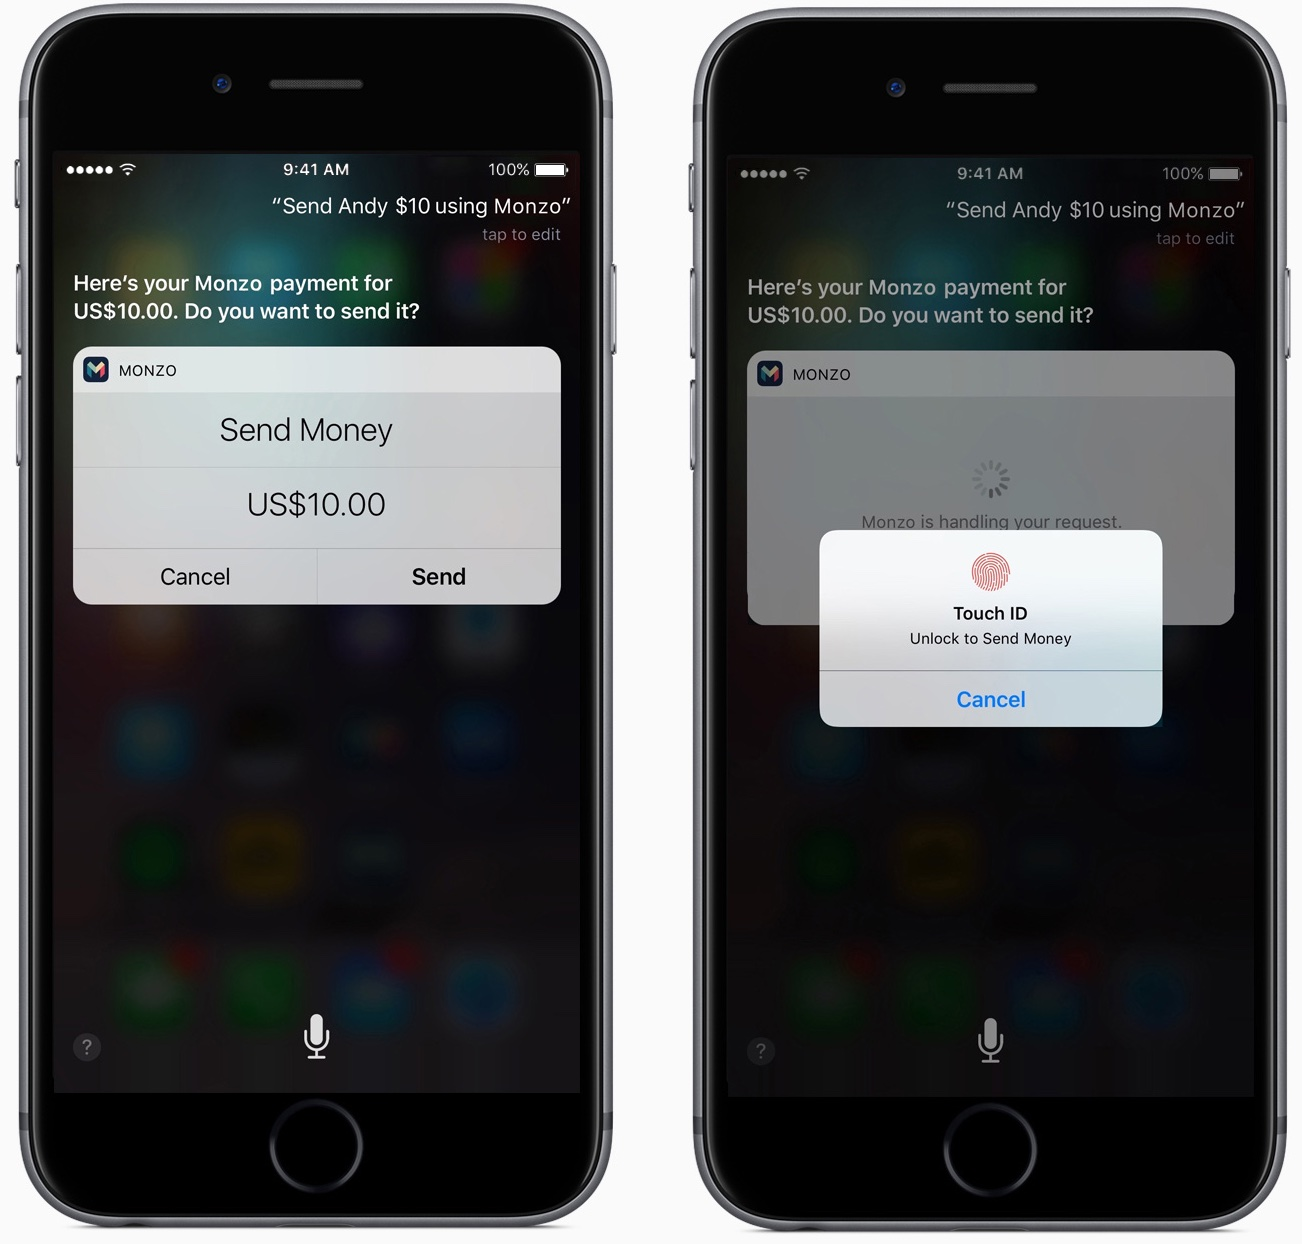
\includegraphics[width=0.5\linewidth]{images/apple_siri/cashconfirm.jpg} 
	\caption{Service paiement 1 \cite{siriDemo}}
\end{figure}

\begin{figure}[H]
	\centering
	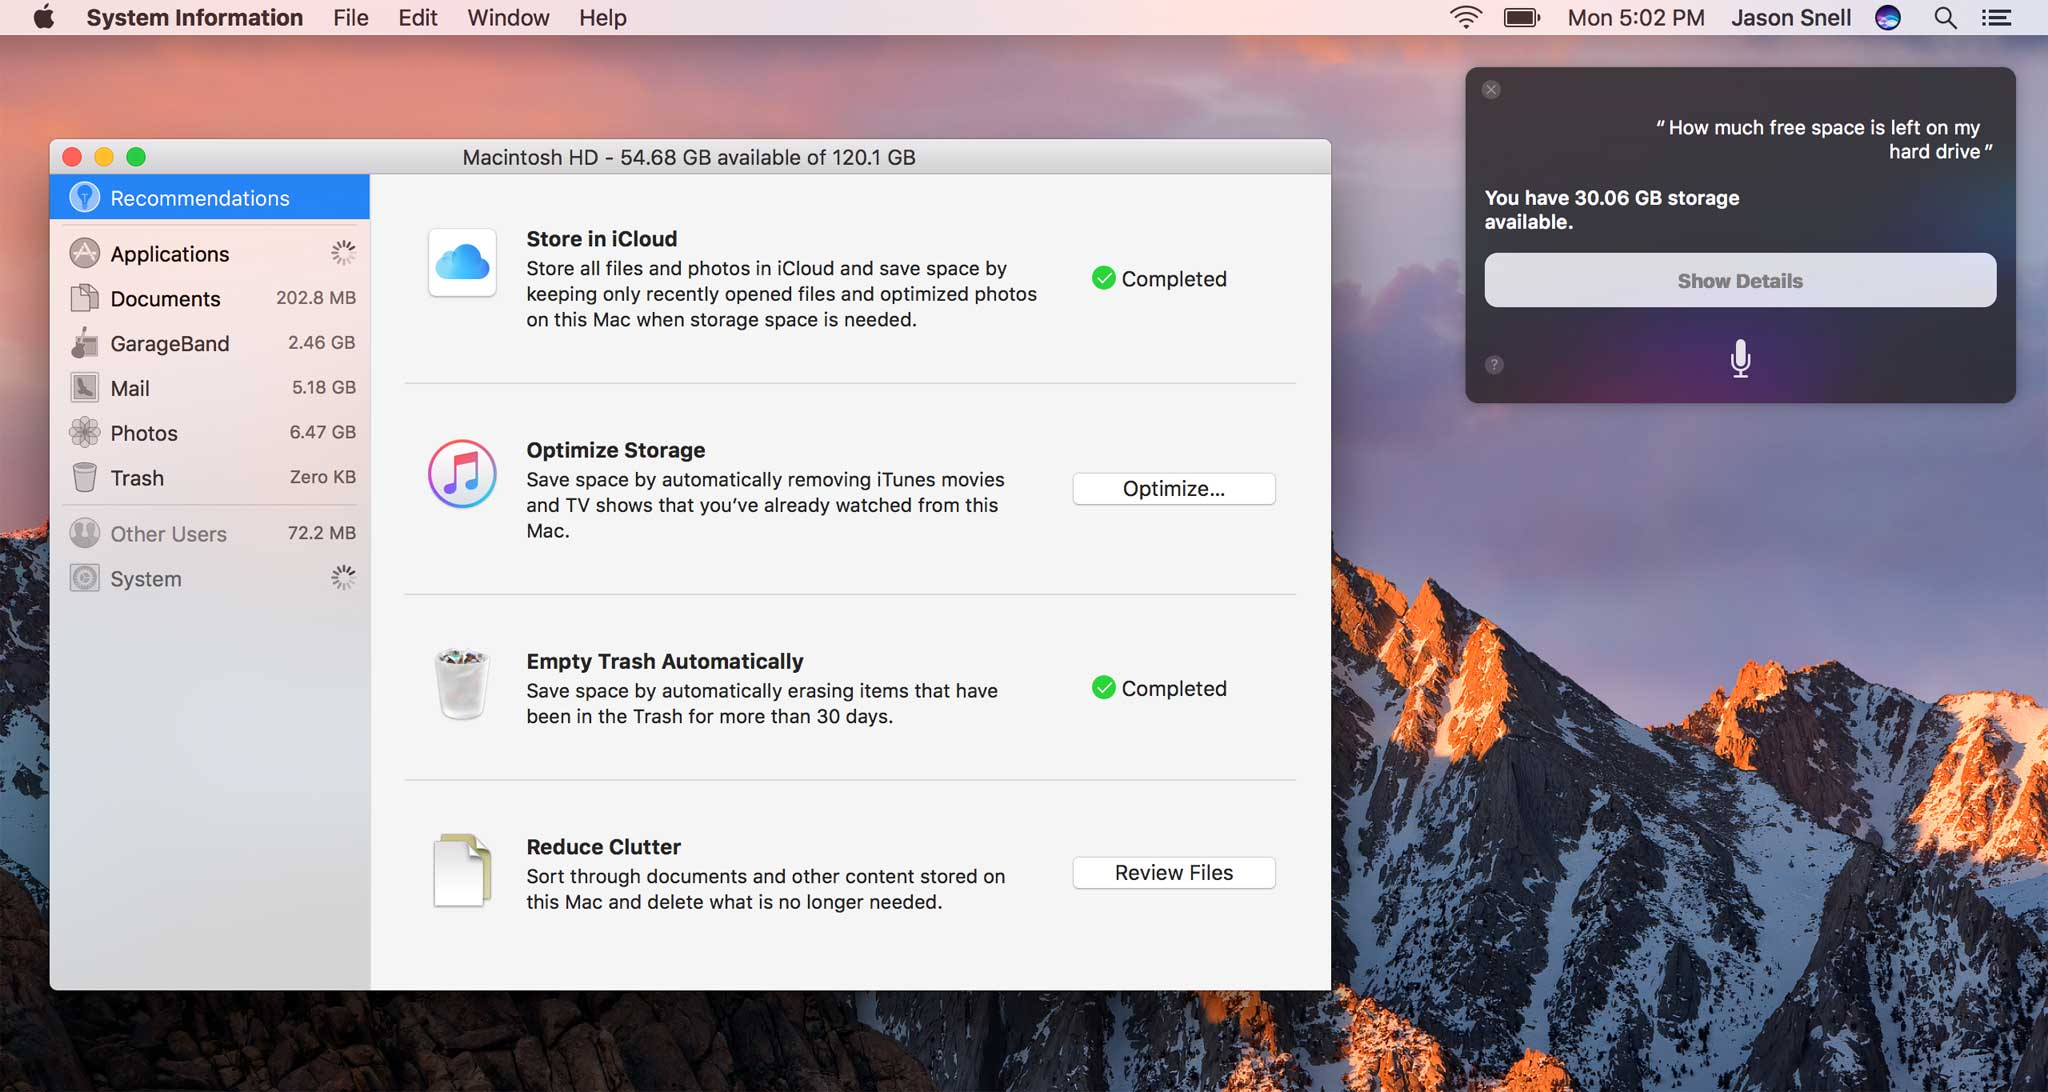
\includegraphics[width=0.75\linewidth]{images/apple_siri/macbook.png} 
	\caption{Siri sur un laptop  \cite{macossiridemo}}
\end{figure}


\subsection*{Amazon Alexa}
\begin{figure}[H]
	\centering
	
\includegraphics[width=.5\linewidth]{images/amazon_alexa/logo.png}
	\caption{Logo d'Amazon Alexa} 
\end{figure}
\paragraph{}Amazon Alexa est un assistant exclusivement intégré au dispositif Amazon Echo(un haut-parleur portatif), à l'instar de Siri, il est aussi capable de communiquer avec l'utilisateur par le biais de la parole, pouvant ainsi executer diverse commandes comme joueur de la musique, réciter des livres audios, annoncer des news en temps réel(Résultats sportifs, tendances politiques ... ), son atout majeur est sa capacité à s'intégrer à plusieurs appareils-connectés(Contrôleur de thermostat ou de lumière ambiantes dans une Smart-House ) ainsi que la possibilité d'ajout de SKILLS(ou compétences) de la part des développeurs tiers pour enrichir la panoplie de services que peut offrir Alexa.
\begin{figure}[H]
	\centering
	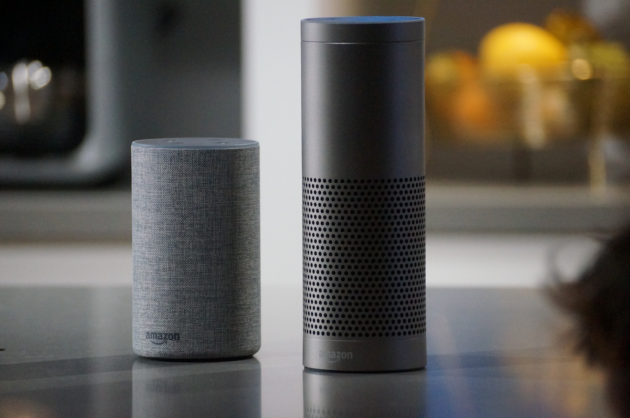
\includegraphics[width=.75\linewidth]{images/amazon_alexa/alexa.png}
	\caption{Haut parleur Echo embarquant l'AVI Alexa} 
\end{figure}
\subsection*{Microsoft Cortana}
\begin{figure}[H]
	\centering
	
\includegraphics[width=.5\linewidth]{images/cortana/logo.png}
	\caption{Logo de Microsoft Cortana} 
\end{figure}
\paragraph{}
Cortana est la tentative de la part de Microsoft d'intégrer un assistant dans son système d'exploitation Windows 10 et WindowsPhone, il propose divers services de base tel que planifier des tâches, exécuter des commandes via la parole, et analyser des résultats de recherche sur le moteur de recherche de Microsoft, a savoir Bing, pour répondre à des questions.
\begin{figure}[H]
	\centering
	
\includegraphics[width=.4\linewidth]{images/cortana/weather.png}
	\caption{Cortana répondant à une requête utilisant Bing } 
\end{figure}

\section{Points fort des AVI's}
\paragraph{}
A travers les sections précédentes ,nous avons appris à découvrir les différents aspect d'un assistants virtuel intelligent, nous avons pu donc apprécié la puissance d'un tel système s'il venait à être perfectionner d'avantage.
\par En effet, en examinant les domaines d'applications, il est facile de déduire que le recours à un AVI peut grandement faciliter certaines tâches, que ce soit pour celles qui sont les plus triviales et donc peuvent retarder d'autres tâches plus importantes, ou bien celles qui doivent faire appel à la précision ou la grande capacité de calcul des machines, assurant ainsi des résultats précis et produits rapidement.


\section{Conclusion}
\paragraph{}
À la fin de ce chapitre nous pouvons donc mettre en valeur la place primordiale que pourrait avoir les AVIs s'ils arrivaient à maturité(c.à.d à briser la barrière qui sépare les humains de la machine et à faire partie de la vie quotidienne des utilisateurs). \par Nous avons d'abord discuté de l'aspect historique des AVIs, ainsi que les caractéristiques essentielles d'un AVI idéal, nous avons ensuite cité quelques domaines d'applications qui leur sont propres, pour ensuite citer quelques exemples d'assistants existants, pour enfin clôturer avec les principaux avantages de tels assistants.
\par Dans le prochain chapitre nous allons principalement aborder les aspects techniques des différents composants de l'AVI que nous désirerions réaliser.

 
